\documentclass[10pt]{article}
\usepackage[margin=1.5cm]{geometry}
\usepackage{graphicx,booktabs,amsmath,amssymb}
\usepackage[hidelinks]{hyperref}
\usepackage{fancyvrb}
\title{Supplementary Material for ``Texture-Invariant Conformal Prediction and Detection in Compound-Gaussian Radar Clutter: Exact Laws, Thermal Noise, and Evaluation on Two Radars''}
\author{M. U. Raza, S. Ahmed, and A. Ahmed}
\date{}
\begin{document}
\maketitle
\noindent All numbers below are generated from the saved outcomes in the project repository (\texttt{research/r7c}). Four protocols were frozen and hash-recorded before their outcomes were computed: the confirmatory IPIX study (\texttt{PROTOCOL.md}), detection (\texttt{detection/PROTOCOL\_DETECTION.md}), baselines (\texttt{baselines/PROTOCOL\_BASELINES.md}) and the second radar (\texttt{jku/PROTOCOL\_JKU.md}).

\section{Hold-out series}
Two further McMaster series (\#269 and \#287, the widely used ``high'' and ``low'' sea-state files, one provider-preprocessed VV cell each, from the same 1993 campaign) were hashed and left unopened until the main analysis was complete, and then evaluated once (Table~\ref{tab:holdout}). They confirm the direction of the main result, with larger gains. They also show a case in which the classical Gaussian threshold over-covers while conformal IN-ARCP stays near nominal. Their test sets are small (about 165 episodes per unit), so the hold-out is a directional check. Mondrian calibration returns infinite regions at $1-\alpha=0.99$ there, because each bin receives fewer calibration episodes than the rank requires.
\begin{table}[h]
\centering\small
\caption{Hold-out series \#269 and \#287 ($1-\alpha=0.90$; six units per column).}
\label{tab:holdout}
\begin{tabular}{lcccc}
\toprule
 & \multicolumn{2}{c}{$m=8$} & \multicolumn{2}{c}{$m=16$}\\
\cmidrule(lr){2-3}\cmidrule(lr){4-5}
Method & Radius ratio & Coverage (min) & Radius ratio & Coverage (min)\\
\midrule
Noise-aware AR(4) (proposed) & 0.454 & 0.890 (0.816) & 0.498 & 0.893 (0.847)\\
Noise-aware AR(2) (proposed) & 0.541 & 0.887 (0.828) & 0.533 & 0.895 (0.859)\\
AR(4), innovation-normalized & 0.546 & 0.908 (0.847) & 0.515 & 0.906 (0.883)\\
AR(2), innovation-normalized & 0.582 & 0.905 (0.840) & 0.572 & 0.906 (0.871)\\
Noise-aware AR(1) & 0.921 & 0.898 (0.840) & 0.921 & 0.903 (0.859)\\
IN-ARCP, AR(1) & 1.000 & 0.906 (0.853) & 1.000 & 0.910 (0.859)\\
Gaussian plug-in of IN-ARCP & 1.178 & 0.949 (0.896) & 1.104 & 0.945 (0.895)\\
Mondrian IN-ARCP & 1.000 & 0.895 (0.804) & 0.981 & 0.896 (0.810)\\
Learned-scale CP & 0.629 & 0.893 (0.804) & 0.662 & 0.919 (0.791)\\
Invariant MLP CP & 1.809 & 0.884 (0.736) & 2.158 & 0.903 (0.761)\\
Raw-RMS normalized CP & 1.321 & 0.880 (0.706) & 1.243 & 0.887 (0.706)\\
Unnormalized CP & 1.142 & 0.868 (0.607) & 1.161 & 0.859 (0.589)\\
Gaussian plug-in of noise-aware AR(4) & 0.411 & 0.866 (0.816) & 0.472 & 0.856 (0.755)\\
\bottomrule
\end{tabular}

\end{table}

\section{Synthetic verification}
\begin{figure}[h]
\centering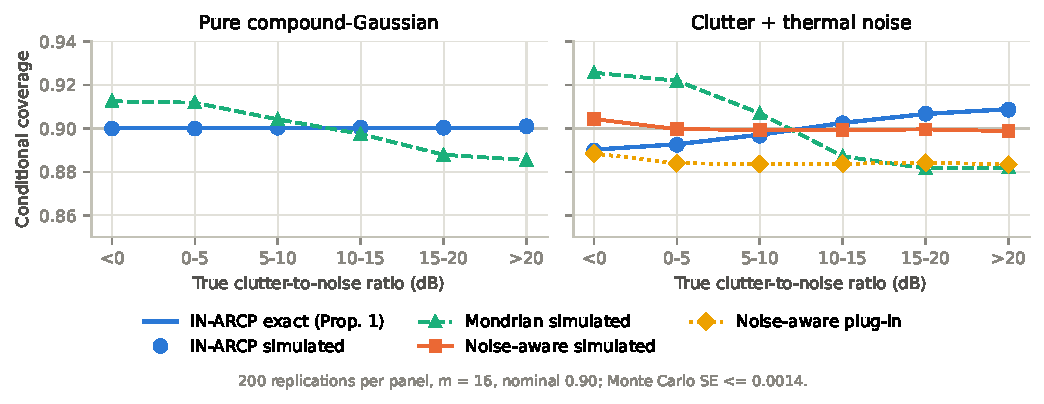
\includegraphics[width=.85\textwidth]{fig_synthetic_exact.pdf}
\caption{Synthetic verification: coverage conditional on the true clutter-to-noise ratio. The line is the exact law of Proposition~1; markers are simulation.}
\end{figure}

\section{Proof sketch of Proposition 4 (zero-noise limit)}
With $\gamma=\nu c$ the history log-likelihood converges locally uniformly on $\gamma>0$ to $-m\log\gamma-\gamma^{-1}h^{\mathsf H}R_H^{-1}h$, whose unique maximizer is $h^{\mathsf H}R_H^{-1}h/m$; coercivity at $0$ and $\infty$ gives convergence of the maximizers. The Markov property gives $\mu\to\rho h_m$, and $(1-|\rho|^2)R_H^{-1}=W_\rho^{\mathsf H}W_\rho$, with $W_\rho$ the bidiagonal whitening matrix, identifies the limiting predictive variance with $s_\rho(h)^2$.

\section{Day transfer and texture-proxy sensitivity}
\begin{table}[h]
\centering\small
\caption{Day transfer ($m=16$, $1-\alpha=0.90$): fit and calibrate on other days, test on each of six held-out days.}
\begin{tabular}{lccc}
\toprule
Method & Mean coverage & Worst held-out day & Radius ratio\\
\midrule
Noise-aware AR(4) (proposed) & 0.898 & 0.863 & 0.936\\
Noise-aware AR(2) (proposed) & 0.898 & 0.883 & 0.956\\
AR(4), innovation-normalized & 0.901 & 0.894 & 0.993\\
AR(2), innovation-normalized & 0.899 & 0.891 & 1.024\\
Noise-aware AR(1) & 0.900 & 0.882 & 1.037\\
IN-ARCP, AR(1) & 0.903 & 0.882 & 1.000\\
Gaussian plug-in of IN-ARCP & 0.906 & 0.893 & 1.006\\
Mondrian IN-ARCP & 0.907 & 0.881 & 0.984\\
Learned-scale CP & 0.898 & 0.774 & 0.967\\
Invariant MLP CP & 0.880 & 0.622 & 1.200\\
Raw-RMS normalized CP & 0.906 & 0.681 & 1.466\\
Unnormalized CP & 0.909 & 0.716 & 1.470\\
Gaussian plug-in of noise-aware AR(4) & 0.876 & 0.842 & 0.893\\
\bottomrule
\end{tabular}

\end{table}
\noindent Texture-proxy sensitivity (pre-specified windows; mean maximum quintile deviation at $1-\alpha=0.90$, $m=16$): with $\pm512$ pulses IN-ARCP 0.035, NA-AR(4) 0.043, unnormalized 0.181, neural centre 0.103; with $\pm2048$ pulses IN-ARCP 0.033, unnormalized 0.141. The ranking is the same as with $\pm1024$.

\section{Additional figures for the IPIX study}
\begin{figure}[h]
\centering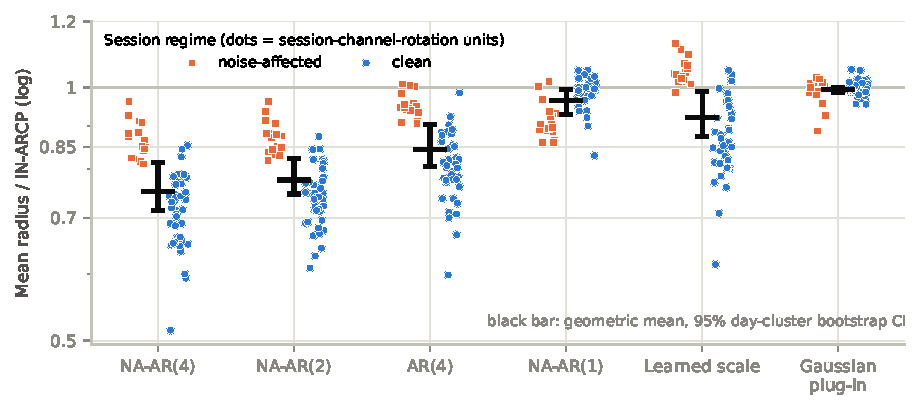
\includegraphics[width=.8\textwidth]{fig_width_ratios.pdf}
\caption{Per-unit radius relative to IN-ARCP at $1-\alpha=0.90$, $m=16$, by session regime (noise-affected: fitted noise power above 1\% of mean power).}
\end{figure}
\begin{figure}[h]
\centering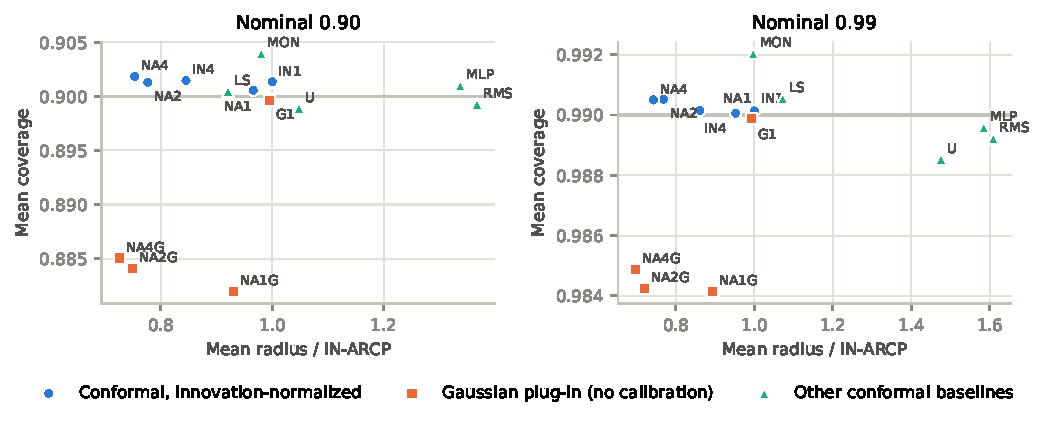
\includegraphics[width=.8\textwidth]{fig_coverage_size.pdf}
\caption{Mean coverage against mean radius (confirmatory, $m=16$). Gaussian plug-ins of the richer noise-aware models are shorter but under-cover; conformal calibration restores nominal coverage. Labels: NA$p$ and IN$p$, noise-aware and innovation-normalized AR($p$) (IN1 is IN-ARCP); G1 and NA$p$G, Gaussian plug-ins; MON, Mondrian; LS, learned scale; U, unnormalized; RMS, raw-RMS; MLP, neural centre.}
\end{figure}

\section{Detection study: all levels and methods}
\begin{figure}[h]
\centering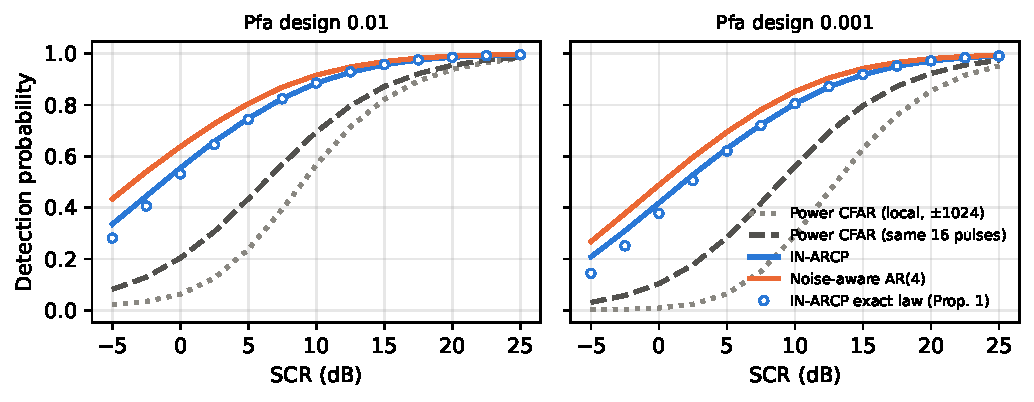
\includegraphics[width=.85\textwidth]{fig_detection.pdf}
\caption{Detection of injected Swerling-1 targets on IPIX at design false-alarm probabilities 0.01 and 0.001.}
\end{figure}
\noindent Pooled detection probability by SCR, measured false-alarm rates, exact-law predictions and SCR gains with 95\% day-cluster intervals (output of \texttt{detection/analyze\_detection.py}):
\VerbatimInput[fontsize=\tiny]{data/detection_summary.txt}

\section{Persistent targets after onset}
Frozen onset study (\texttt{detection/PROTOCOL\_ONSET.md}): per-look detection probability, cumulative detection within $K$ looks, and clean cumulative false-alarm probabilities:
\VerbatimInput[fontsize=\tiny]{data/onset_summary.txt}
\noindent Exploratory: comparison at equal dwell false-alarm probability (0.01), with max and sum-of-squares dwell statistics:
\VerbatimInput[fontsize=\tiny]{data/dwell_summary.txt}
\noindent Exploratory: exact-law prediction of the post-onset decay:
\VerbatimInput[fontsize=\tiny]{data/onset_theory.txt}

\section{Numerical checks of the detection theory}
Monte Carlo checks of Corollary~2, Proposition~2 (closed forms) and Proposition~3 (output of \texttt{detection/theory\_checks.py}):
\VerbatimInput[fontsize=\tiny]{data/theory_checks_output.txt}

\section{Baselines: parametric texture and adaptive conformal inference}
\VerbatimInput[fontsize=\tiny]{data/baselines_summary.txt}

\section{Second radar: full results}
\begin{figure}[h]
\centering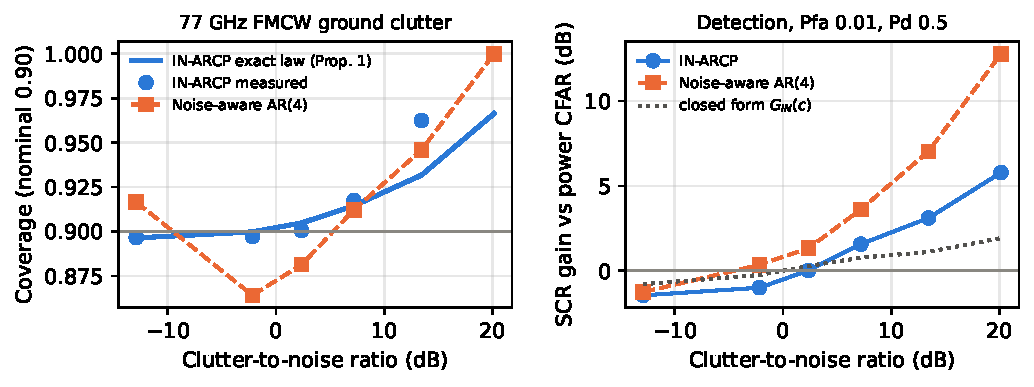
\includegraphics[width=.85\textwidth]{fig_jku.pdf}
\caption{77~GHz FMCW ground clutter: coverage by CNR class with the exact law, and SCR gain over the local power detector.}
\end{figure}
\VerbatimInput[fontsize=\tiny]{data/jku_summary.txt}
\end{document}
